\section{Testing, Cleaning and Commissioning} \label{sec:Testing}\label{sec:Commissioning}
CALIS was assembled at FNAL from components produced at FNAL and at the University of Hawaii. After initial basic functionality tests at FNAL, CALIS was shipped pre-assembled to LNGS, where it underwent a comprehensive testing and calibration program. While still outside the clean room CRH, CALIS was installed on a high bay platform in the LNGS underground Hall C and tested to its full deployment length. Besides testing basic $z$-motion, articulation and $xy$-rotation, all details of CALIS operations were tested. These included the testing of the functionality of motor controls, the high limit and articulation switch. Validation was concluded with recovery scenarios after, e.g.,~power failures during deployment.

An important aspect was $z$-position calibration of the source as a function of cable length before and after source arm articulation, which is a nonlinear function of motor step counts, as mentioned in Sec.~\ref{sec:Nonlinearity:MotorStepCounts}. Furthermore, the source's $xy$- and $z$-position accuracy and precision were estimated.

This testing campaign's results were reviewed by an internal review board and approval for installation of CALIS inside CRH was granted. CALIS was cleaned according to official cleaning procedures and installed on its gate valve in September 2014.
After installation on the gate valve a testing focus was the system's light and helium leak tightness, as well as validation of nitrogen and vacuum systems, as these could only be tested fully after installation. A more detailed description of tests performed at FNAL and LNGS can be found in \cite{thesis:Hackett, thesis:Edkins}.

\subsection*{$xy$- and $z$-position}
Tests in air and in the LSV's scintillator revealed that the dominant source of uncertainty in the source position arises during articulation. Positioning in $z$ before articulation is highly accurate and precise: deployment speed is very low, barely visible to the naked eye (0.4 cm/s), which minimizes lateral motion and avoids contact with the housing or the organ pipe during deployment. Yet during articulation a swing of the source in $xy$ arises from tiny laterally imbalanced forces originating in the cable manipulated for articulation. 

To ensure deployment precision, a procedure has been worked out to make reliably gentle contact with the cryostat, thereby eliminating precision uncertainty in $xy$: After positioning the deployment device in $z$, the source arm is articulated to horizontal while it is still pointing away from the cryostat. Only then is the source brought into contact with the cryostat through an $xy$-rotation of the upper assembly, while monitoring scaler rates in the TPC's photomultiplier tubes (PMT).  These increase while the source is approaching, yet plateau as soon as contact with the cryostat is made, even if $xy$-rotation continues. This procedure provides a reliable $xy$- and $z$-position for the calibration source and was used throughout all calibration campaigns.

%%%%%%%%%%%%%%%%%%%%%%%%%%%%%%%%%%%
%%%%%%%%%%%%%%%%%%%%%%%%%%%%%%%%%%%

\section{Calibration Campaigns}\label{sec:CalibCampaigns}
\subsection{Radioactive Sources}
For the calibration of the \lsv\ detector response and the \tpc's response to electron recoils (ER), $^{57}$Co, $^{133}$Ba and $^{137}$Cs were selected. $^{22}$Na was deployed in a later calibration campaign. They allow a cross-calibration with $^{83m}$Kr that was injected into the LAr recirculation system during dedicated campaigns and internal $^{39}$Ar inherent to AAr, as they cover the $^{39}$Ar energy range (see also Table~\ref{tbl:GammaSources} and Fig.~\ref{fig:GammaSources_Ar39spectrum}). %As the interaction length increases with energy in LAr, the different gamma sources allow also to probe different regions of the TPC active volume.  

After a preselection of gamma source energies, detailed studies with the DarkSide Monte Carlo (MC) simulation package G4DS \cite{DS50:G4DS:paper} were performed to select appropriate source activities and to check the feasibility and physics reach of various deployment positions. Sources with suitable activities were identified for deployment considering also constraints from the \lsv\ and \tpc\ DAQs (Table~\ref{tbl:GammaSources}).

Energy variables are calibrated in photo-electrons (PE) using dedicated laser calibration runs, in which each PMT's single PE charge spectrum is fitted and a PE-charge gain is determined. 
These laser runs are also an integral part of all calibration campaigns, which require a laser run every few hours and after each change in DAQ, \tpc\ or CALIS configuration, such as drift field changes or source position changes.

\begin{figure}[htbp]
 \centering
 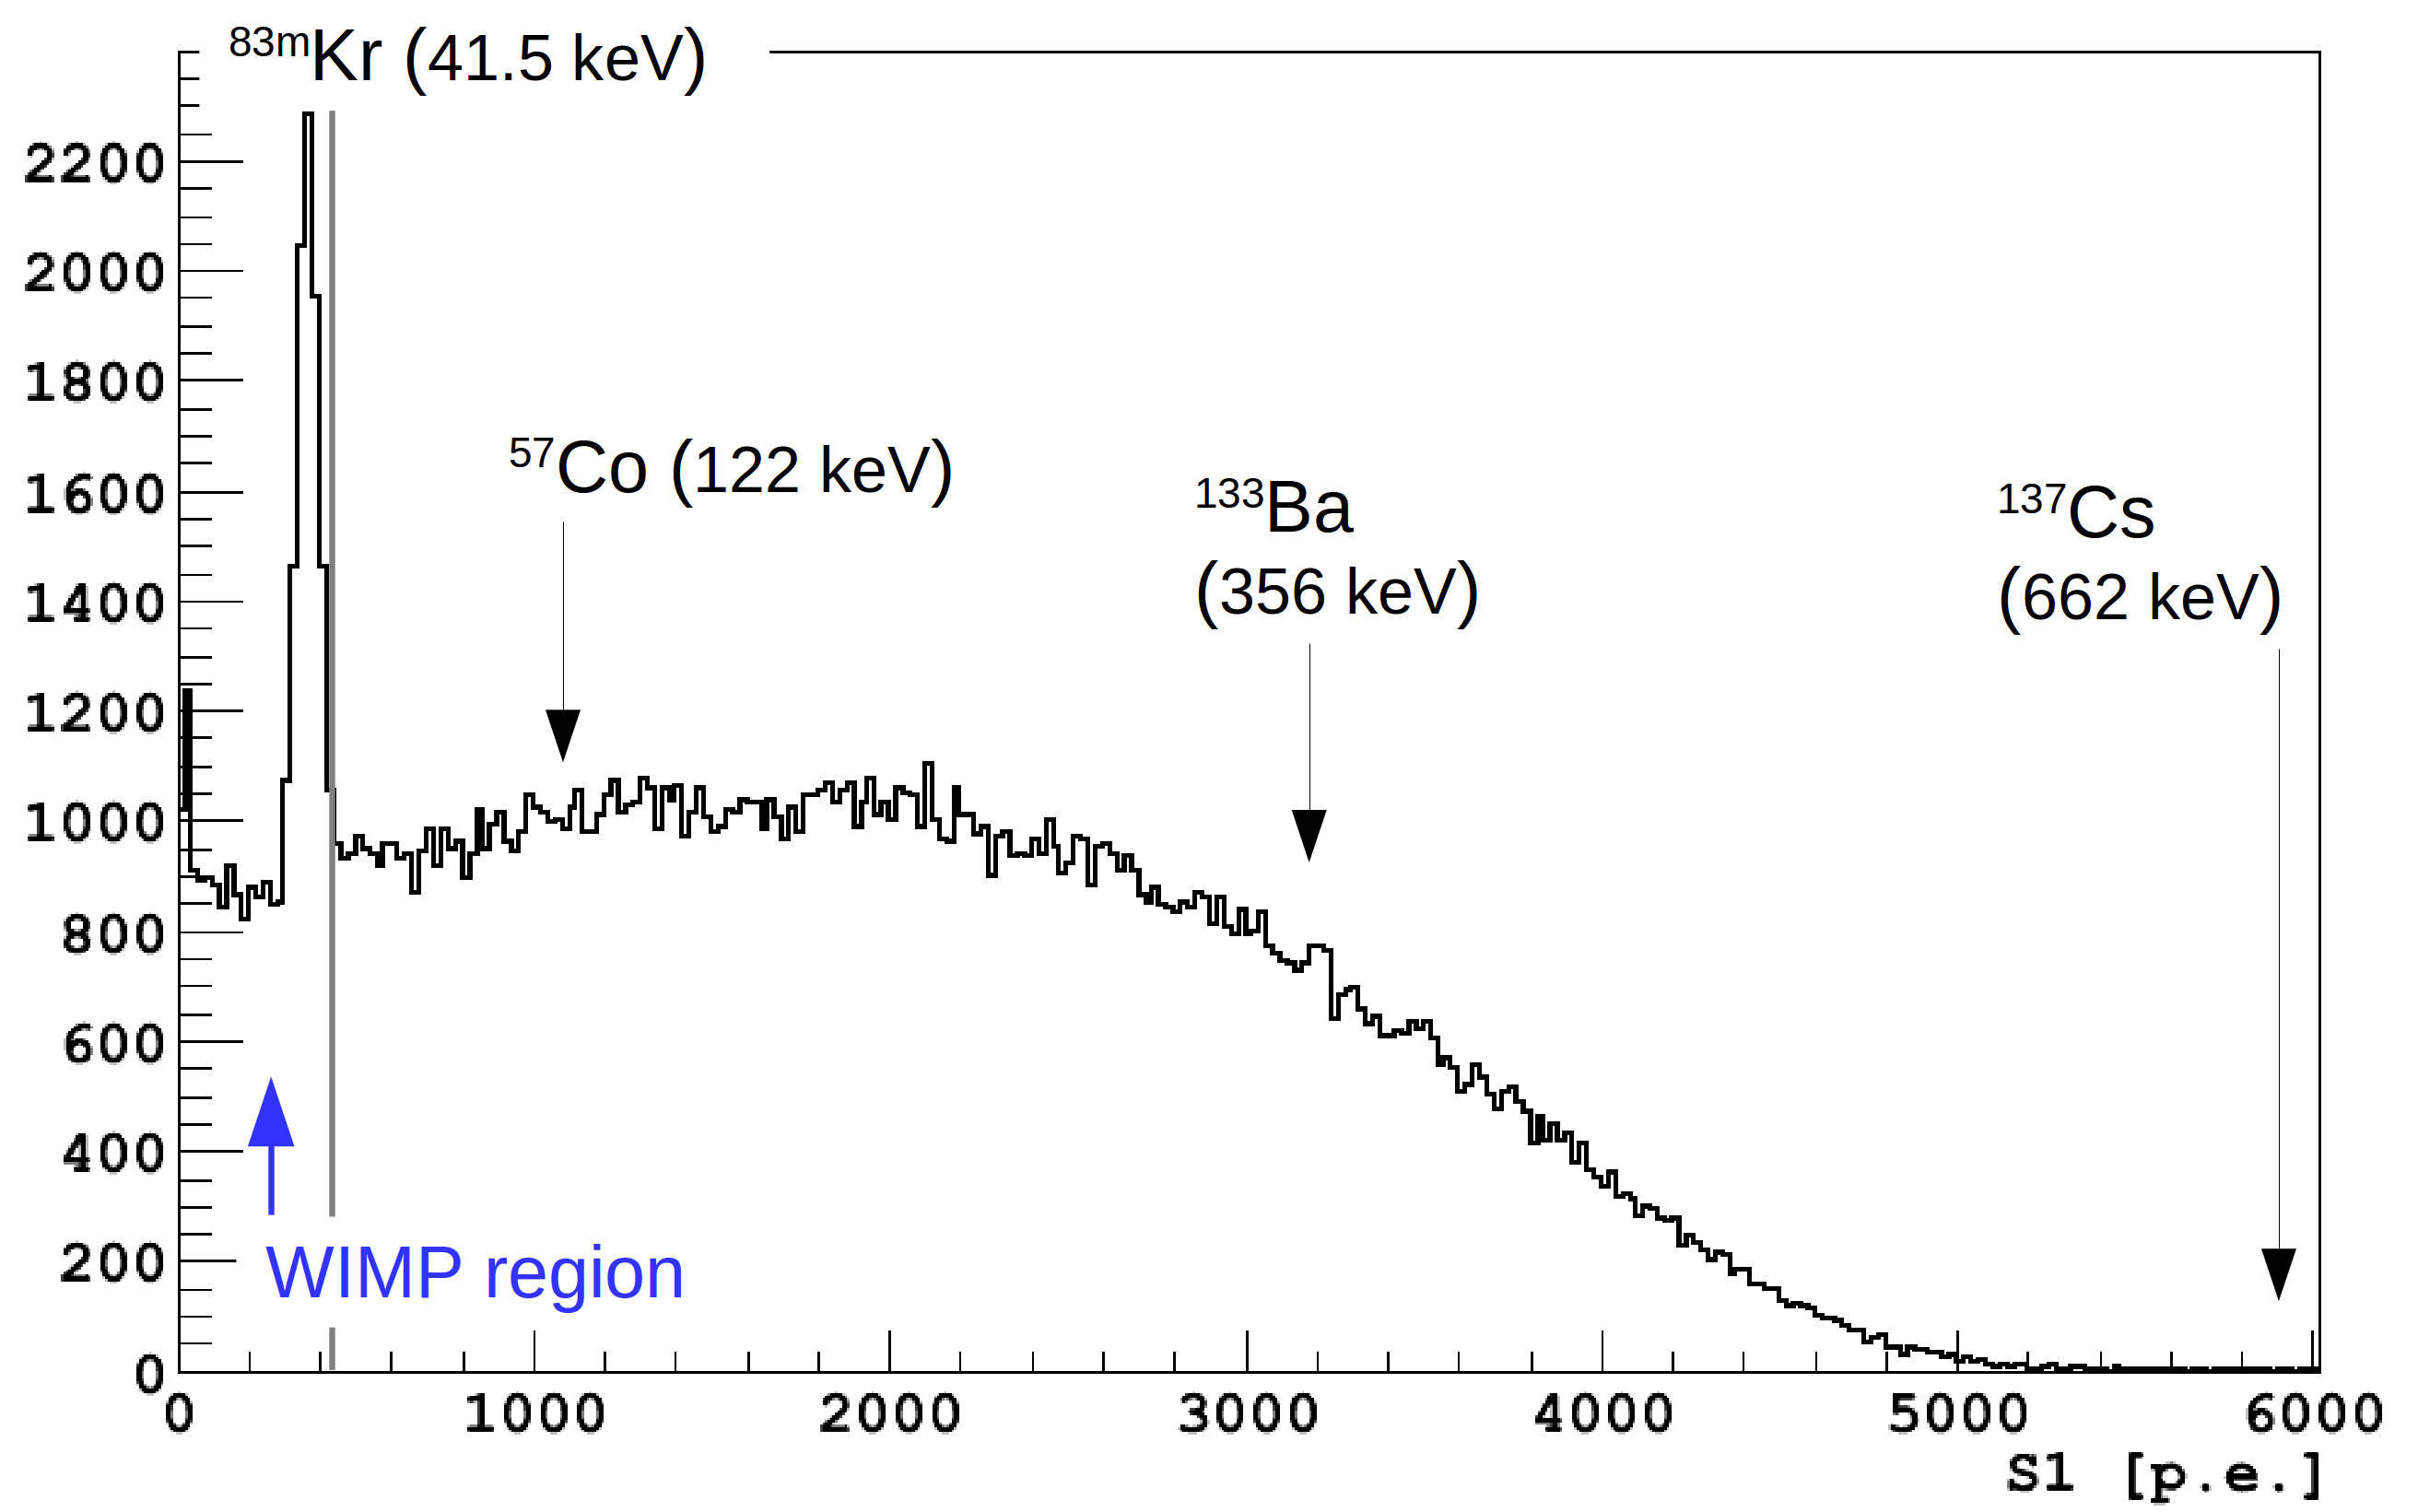
\includegraphics[width=0.8\textwidth]{Figures/GammaSources_Ar39spectrum.png}
 \caption{The AAr scintillation spectrum (S1) at null field showing a $^{83m}$Kr peak on top of the internal $^{39}$Ar $\beta$-spectrum inherent to AAr. The positions of full absorption peaks of three gamma sources are indicated and cover the full range of the $^{39}$Ar spectrum.
\label{fig:GammaSources_Ar39spectrum}}
\end{figure}

\begin{table}[htbp]
\centering
\caption{Gamma sources deployed in DS-50, the internal $^{39}$Ar and the $^{83m}$Kr source. The $^{83m}$Kr atoms are produced in decays of $^{83}$Rb which have a half-life of 86.2 days. The $^{83m}$Kr decays with a half-life of 1.8 hours, emitting 32.1 keV and 9.4 keV conversion electrons \cite{Lippincott:2010jb}. The Kr source activity varied from campaign to campaign, due to the relatively short half-life of $^{83}$Rb, yet it was in the range of a few Bq to some tens of Bq. The $^{39}$Ar activity has been approximately 50 Bq (1 Bq/kg) during AAr filling and negligible in the UAr phase.} %\cite{Lippincott:83mKr}
\centering
\begin{tabular}{|l|l|l|l|l|}
\hline
\textbf{source} & \textbf{type} & \textbf{energy} & \textbf{half life} & \textbf{activity} \\ \hline
$^{57}$Co & $\gamma$ & 122 keV & 0.744 y  & 35 kBq \\ \hline
$^{133}$Ba & $\gamma$ & 356 keV & 10.54 y & 2 kBq \\ \hline
$^{137}$Cs & $\gamma$ & 662 keV & 30.2 y & 0.65 kBq \\ \hline
$^{22}$Na & $\gamma$ & $2\cdot 511$ keV + 1274 keV & 2.603 y & 11 kBq \\ \hline\hline
$^{39}$Ar & $\beta$ &  565 keV endpoint& 269 y  & 50 Bq\\ \hline
$^{83m}$Kr & 2 $\beta$ &  32.1 keV + 9.4 keV & 86.2 d & varying\\ \hline
\end{tabular}
\label{tbl:GammaSources}
\end{table}

%\begin{tabular}{|l|l|l|l|l|l|}
%\hline
%\textbf{source} & \textbf{type} & \textbf{energy} & \textbf{half life} & \textbf{interact. length} & \textbf{activity} \\ \hline
%$^{57}$Co & $\gamma$ & 122 keV & 0.744 y & 4.4 cm & 35 kBq \\ \hline
%$^{133}$Ba & $\gamma$ & 356 keV & 10.54 y & 7.5 cm & 2 kBq \\ \hline
%$^{137}$Cs & $\gamma$ & 662 keV & 30.2 y & 9.5 cm & 0.65 kBq \\ \hline
%$^{22}$Na & $\gamma$ & $2\cdot 511$ keV + 1274 keV & 2.603 y & 8.4/ 11.3 cm & 11 kBq \\ \hline\hline
%$^{39}$Ar & $\beta$ &  565 keV endpoint& 269 y & sub-mm & 50 Bq\\ \hline
%$^{83m}$Kr & 2 $\beta$ &  32.1 keV + 9.4 keV & 86.2 d & sub-mm & varying\\ \hline
%\end{tabular}
%\label{tbl:GammaSources}


\subsection{Calibration Campaigns Timeline and Stability}
The following calibration campaigns were performed between October 2014 and April 2016:
\begin{itemize}
\item The first extensive campaign involving all gamma sources and both a high and low activity \AmBe\ neutron source took place in October and November 2014 at LNGS. The \tpc\ was filled with AAr with an inherent trigger rate of approx. 50 Hz from $^{39}$Ar. The \lsv's liquid scintillator consisted of PC, with $<0.1 \%$ TMB and 1.4 g/l PPO as wavelength shifter \cite{Agnes:2015qyz}.
%Fig.~\ref{???} shows the different configurations in which data has been taken as a function of source energy, source position and drift field.

\item A second campaign focusing on \lsv\ calibration using the low activity \AmBe\ source was performed in January and February 2015. Before this campaign, the \lsv\ was reconstituted with 5\% TMB. Two deployments were performed at two different PPO concentrations (0.7 g/l and 1.4 g/l), allowing the study of the impact of the PPO concentration on alpha and gamma quenching. (1.4 g/l is our nominal PPO concentration, see also Fig.~\ref{fig:LSV:Calib}, right.)
\item A $^{22}$Na source was deployed next to the cryostat for TPC calibration in August 2015. This was the first gamma source calibration campaign after the deployment of UAr within \dsf.
\item An \AmC\ neutron source was deployed in December 2015, allowing an in-depth study of the detection efficiency of the prompt neutron thermalization signal, which is obfuscated in a majority of \AmBe\ decays by its neutron-correlated high energy gamma.
\end{itemize}

In dedicated analyses it has been shown that the calibration campaigns have not negatively affected the light yield so far or introduced additional radioactivity into the \lsv\ \cite{Agnes:2015qyz}.

%\begin{figure}[htbp]
%\centering
%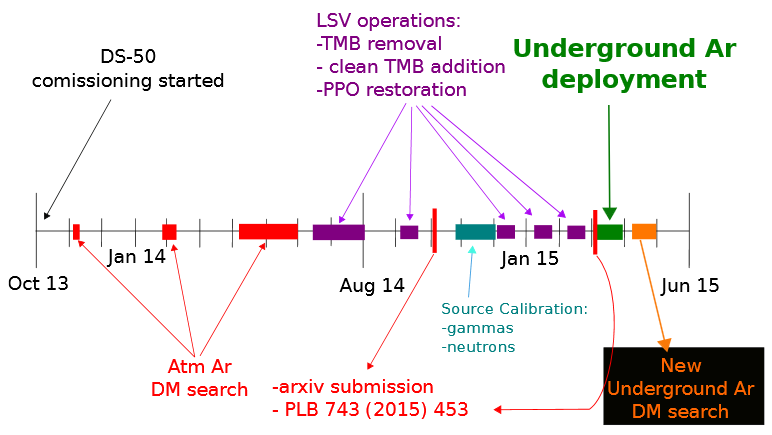
\includegraphics[width=0.7\textwidth]{./Figures/Yann_timeline.png}
%\caption{In black the stability of the LSV LY is monitored using internal $^{60}$Co emitted from the cryostat steel, in blue the stability %of the rate of radioactivity in the LSV is shown. Before and after calibration campaigns both the LY and the rate remain unaffected.
%\label{fig:LSV:Stability}}
 %\end{figure}


\subsection{TPC Calibration}
A few calibration results are shown illustrating the quality of acquired calibration data and the high level of agreement with their description in the G4DS MC package.

\subsubsection{$^{57}$Co Scintillation Energy}
Fig.~\ref{fig:CalibData:Co57} shows a data-MC comparison of the scintillation signal spectrum (S1) of a $^{57}$Co calibration source deployed next to the cryostat and close to the TPC active volume center in $z$. The S1 distribution is overlayed by an equivalent selection of G4DS MC simulation events.\mymarginpar{The plot is from Paolo's G4DS talk \@ DS2016, UCLA. Ideally one could get an official copy from the MC paper.}

\begin{figure}[htbp]
\centering
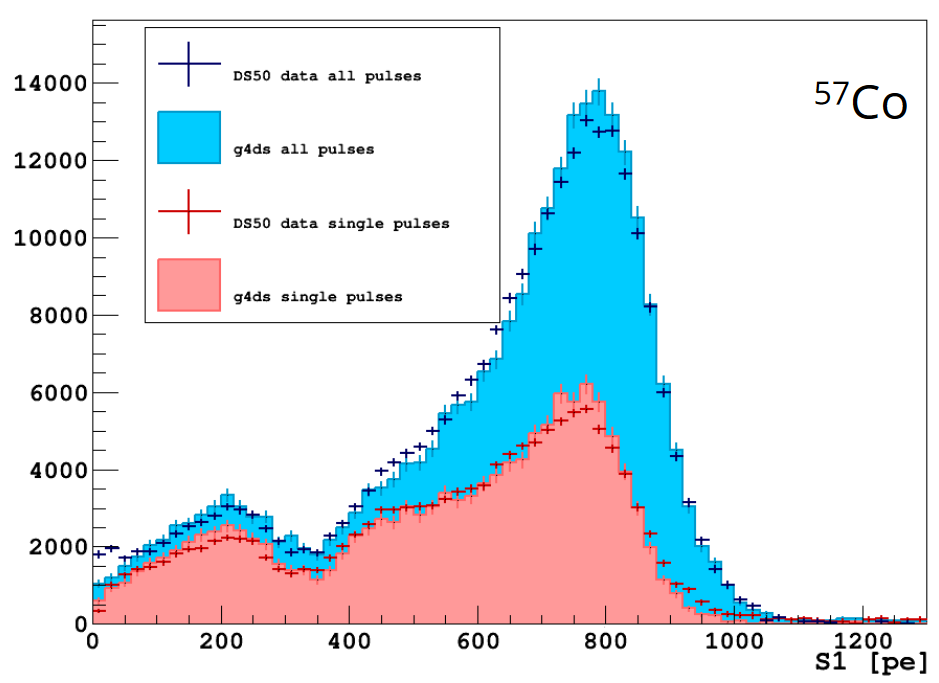
\includegraphics[width=0.6\textwidth]{./Figures/57Co_Paolo_G4DS_UCLA.png}
\caption{Data-MC comparison for a $^{57}$Co source deployed next to the cryostat. In the magenta distribution a single-site interaction requirement is imposed as for dark matter events and for the blue distribution this constraint is removed \cite{DS50:G4DS:paper}.
\label{fig:CalibData:Co57}}
 \end{figure}


\subsubsection{\FNinety\ distribution from $^{241}$Am$^9$Be neutron data}\label{sec:CalibData:NR}

Fig.~\ref{fig:CalibData:F90} shows good agreement between \FNinety\ medians and the S1 spectra measured from $^{241}$Am$^9$Be neutron data in the \dsf\ \tpc\ and those derived from \SCENE\ measurements \cite{Agnes:2015_uar}. The latter have been used to determine the nuclear recoil energy scale and NR acceptance regions for the \dsf\ WIMP dark matter searches \cite{Agnes:2015gu, Agnes:2015_uar}.
\begin{figure}[htbp]
\centering
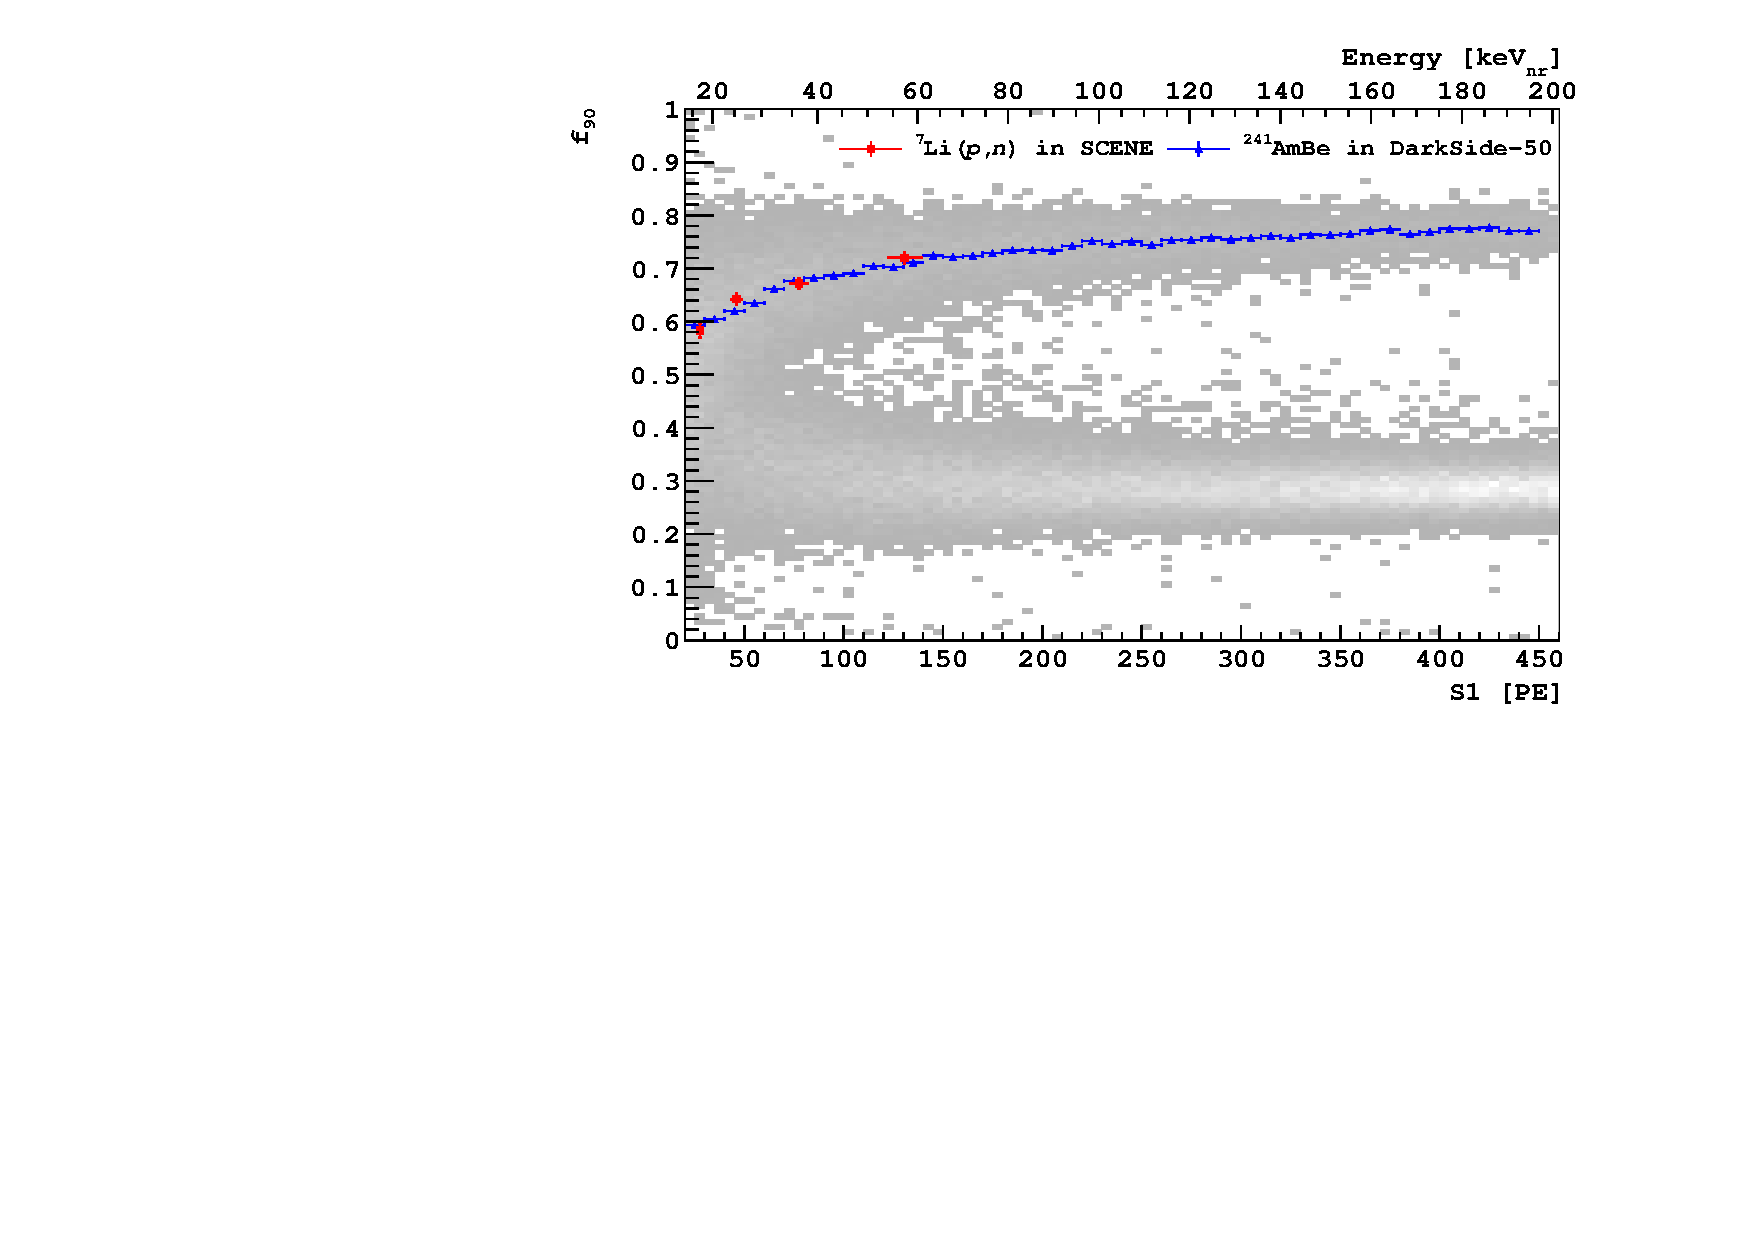
\includegraphics[width=0.7\textwidth]{./Figures/DSf-UArAmBeDMSStCut.pdf}
\caption{Plot of \FNinety\ vs.~the scintillation signal S1 from a high rate {\it in situ} \AmBe\ neutron source calibration of \dsf\ in grey. The upper NR band from the \AmBe\ calibration and lower ER band from $\beta$-$\gamma$ backgrounds are visible. Overlaid are the \FNinety\ \NR\ medians vs.~\SOne\ from the \AmBe\ calibration (blue) and those scaled from \SCENE\ measurements (red points) \cite{Cao:2015ks}. There is very good agreement between the two.  High source intensity and correlated neutrons and $\gamma$-ray emissions by the \AmBe\ source contribute events outside the nuclear recoil and electron recoil bands (reproduced from \cite{Agnes:2015_uar}).\label{fig:CalibData:F90}\label{fig:DSf-UArAmBeDMS}} 
\end{figure}


\subsubsection{Source position}\label{sec:SourcePosition}
Tests at LNGS established the deployment system's source positioning accuracy to be about $\pm$1 cm after a 7 meter journey into the \dsf\ \lsv.
%comment to the "about $\pm ": the tilde $~ \pm$ did not show up at all in the output.
During the first calibration campaign several runs have been taken with the source at its central position. %(731000 motor step counts)
Fitting the \tdrift\ distribution at that position for a sequence of runs, a systematic shift vs.~time has been observed (Fig.~\ref{fig:SourcePosition}, right). The source position has been on average 157.4 mm below the TPC extraction grid with an RMS of 10.1 mm. Following that observed systematic shift with time, the deployment procedures were revised to avoid such a time dependency in the future and to improve the deployment precision: Prior to moving the source to its target position, the deployment device is sent to its lowest position, where cables are fully unwound and any asymmetric build-up in the cables is released. It is worth mentioning that this source position imprecision does not induce significant uncertainties for calibration data analyses, as the \tdrift\ distribution can be measured in-situ on a per-run basis and offsets can be corrected for.
\begin{figure}[htbp]
\centering
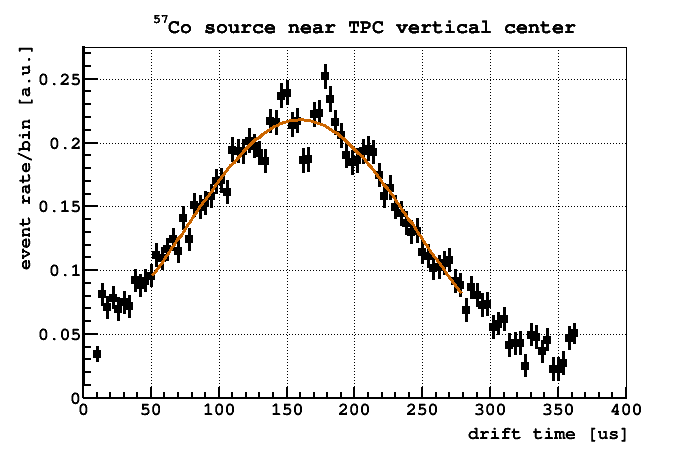
\includegraphics[width=0.48\textwidth]{./Figures/Tdrift_distribution_Co57.png}
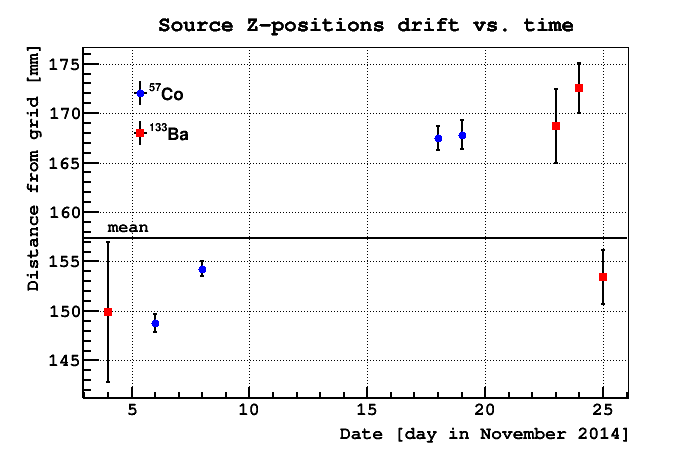
\includegraphics[width=0.48\textwidth]{./Figures/SourcePosition_vs_time.png}
\caption{\textit{Left:} A \tdrift\ distribution encoding the $z$-position of a $^{57}$Co source deployed next to the TPC vertical center. Single scatter events have been selected and a background distribution has been statistically subtracted. Fluctuations in the otherwise smooth \tdrift\ distribution are from copper field cage rings surrounding the TPC.
\textit{Right:} Shift of the source position relative to the TPC extraction grid as measured from the \tdrift\ distribution as a function of time when deployed to the same target position.
\label{fig:SourcePosition}} 
\end{figure}

For the $xy$-position of the calibration source, distributions of the azimuthal angle in the $xy$-plane have been studied and a 139 degree mean was observed with a 1.2 deg RMS. (One degree corresponds to 6 mm at the outer cryostat, where the source is positioned.) However, an independent $xy$ reconstruction algorithm gave 142.5 degrees with an RMS of 0.8 deg, so that systematic uncertainties from the reconstruction algorithm dominate over the $xy$ positioning precision. %\cite{DS:XY:paper}.
\mymarginpar{This is from DocDB 1288. Ideally one could cite a $xy$ paper here, which is not published yet.}


%%%%%%%%%%%%%%%%%%%%%%%%%%%%%%%%

\subsection{Liquid Scintillator Veto}\label{sec:LSV:gammasources}

In Fig.~\ref{fig:LSV:Calib} (left) a data-MC comparison of the LSV charge spectra from a $^{137}$Cs source deployed in the LSV next to the cryostat is shown \cite{DS50:G4DS:paper}.
In January and February 2015, the LSV scintillator reconstitution was completed and a second LSV calibration using an \AmBe\ neutron source was undertaken to further study various LSV neutron detection channels. With a borated scintillator, a critical aspect of the neutron detection efficiency is the capability to observe the \brbortenground\ capture branch leading to a \enbortengroundalpha\ $\alpha$ + $^7$Li(g.s.) without the accompanying 478 keV $\gamma$-ray. As shown in Fig.~\ref{fig:LSV:Calib} (right), the de-excitation channel is clearly observed at around 30 PE.

\begin{figure}[htbp]
\centering
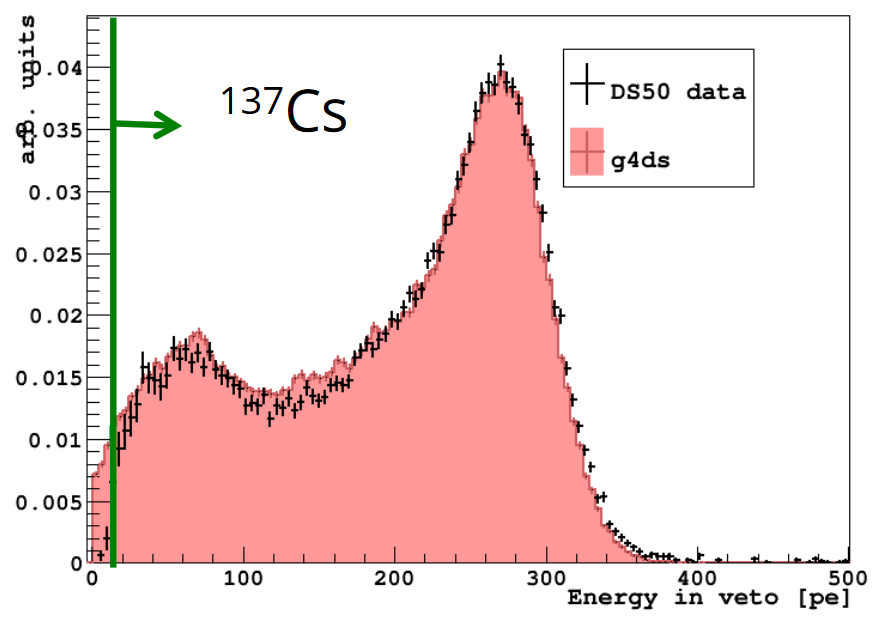
\includegraphics[width=0.44\textwidth]{./Figures/137Cs_Veto_Paolo_G4DS_UCLA}
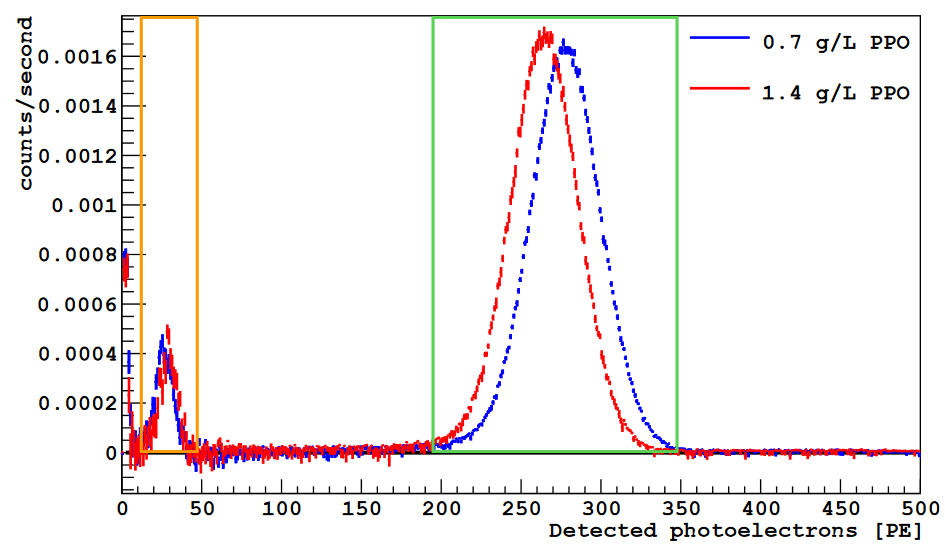
\includegraphics[width=0.54\textwidth]{./Figures/AmBe_LSV_VetoPaper}
\caption{\textit{Left:} A data-MC comparison of the $^{137}$Cs source LSV charge spectrum while the source was deployed next to the cryostat \cite{DS50:G4DS:paper}.
\textit{Right:} A clear detection signal of the neutron capture on $^{10}$B in the LSV. The peak at $\approx$ 30 PE on the left (orange box) is due to a \enbortengroundalpha\ $\alpha$ + $^7$Li(g.s.). The peak on the right at $\approx$ 270 PE (green box) is from 93.6~\% of captures that lead to the $^7$Li excited state reaction, with the accompanying 478 keV $\gamma$-ray. The entries below 10 PE are due to PMT after-pulses. Data has been taken before and after varying the PPO wavelength shifter concentration in the scintillator with the \AmBe\ source rotated away by 90$^{\circ}$ from the cryostat. Though the additional PPO reduced the light yield a bit, it also reduced the quenching of the critical alpha, as expected. Thus at both PPO concentrations the de-excitation to ground state is clearly observed \cite{Agnes:2015qyz}.
\label{fig:LSV:Calib}} 
\end{figure}